\section{绘图命令}
SAC提供了许多与绘图有关的命令,包括控制图像外观的参数控制类命令以及执行绘图功能
的操作执行类命令。这一节将一一介绍操作执行类命令。

\subsection{plot}
plot命令在一个窗口中每次只显示一个波形,并在每两个波形之间暂停以等待用户的输入。
该命令的具体用法在第~\ref{subsec:plot}节已经详细介绍。

\subsection{plot1}
plot1命令在一个窗口中显示多个波形,这些波形共用一个X轴(时间轴),但拥有单独的Y轴。
该命令的绘图效果如图~\ref{fig:plot1}所示。

当一次性读入多个波形数据时,若直接使用plot1绘图,会导致一个窗口内有太多
波形,反而什么都看不清,plot1提供了额外的选项和参数以指定一个窗口内最多显示
多少个波形,余下的波形则处于等待状态。
\begin{SACCode}
SAC> dg sub local cdv.[enz] cvl.[enz] cvy.[enz]  // 生成9个地震波形
cdv.e cdv.n cdv.z cvl.e cvl.n cvl.z cvy.e cvy.n cvy.z
SAC> p1 p 3         // p是选项perplot的简写,3代表每次显示3个波形
Waiting
Waiting
SAC> 
\end{SACCode}
经常遇到的情况是,想要将每个台站的三分量波形记录放在一起看,这个时候设置选项perplot的参数值为3即可。

\subsection{plot2}
plot2会在一个窗口内绘制多个波形,波形同时共用X轴和Y轴。

\begin{SACCode}
SAC> fg seis                     // 生成数据
SAC> rmean; rtrend; taper        // 预处理
SAC> w seis.0                    // 写入滤波前文件
SAC> bp c 0.05 10 n 4 p 2        // 滤波
SAC> w seis.1                    // 写入滤波后文件
SAC> r ./seis.[01]               // 读入两个文件
./seis.0 ...seis.1
SAC> color red inc list red blue // 设置颜色
SAC> p2                          // 绘图
\end{SACCode}
图~\ref{fig:plot2}~中红线为滤波前波形,蓝线为滤波后波形,二者共用X轴和Y轴。

plot2适合做多个波形的对比,常用于数据处理前后波形对比或真实波形与合成波形间的对比。

\begin{figure}[H]
\centering
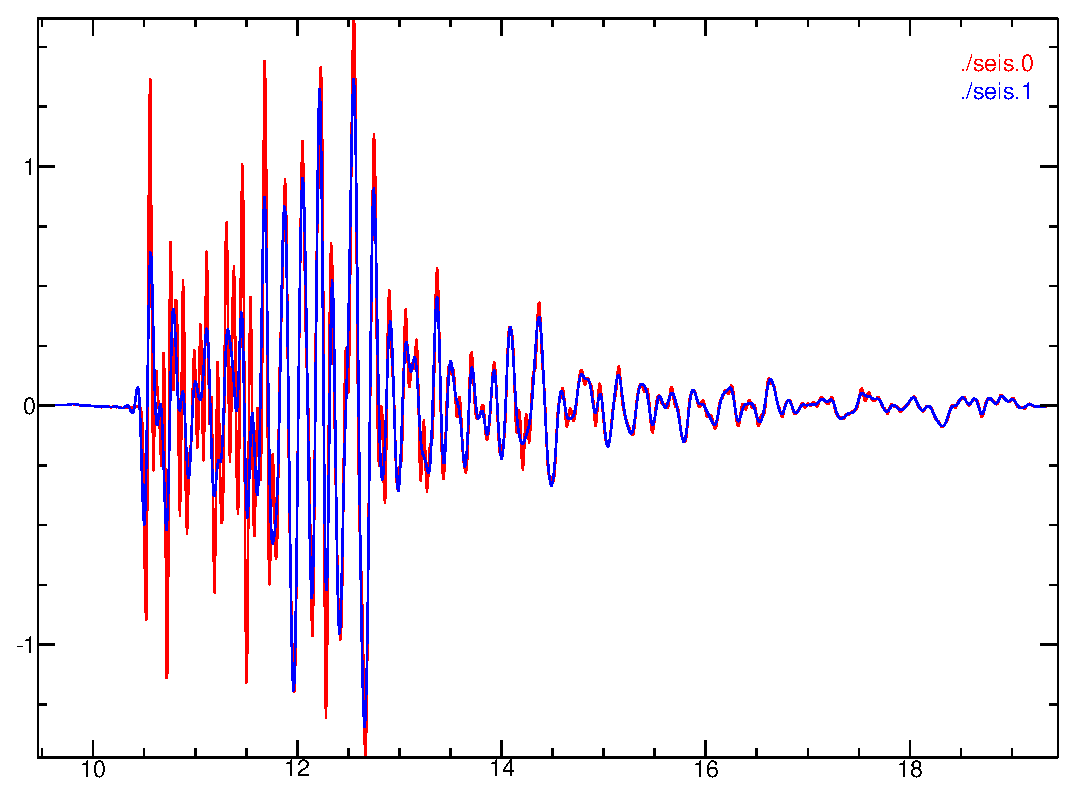
\includegraphics[width=\textwidth]{plot2}
\caption[plot2绘图效果]{plot2绘图效果。红色为滤波前波形,蓝色为滤波后波形。}
\label{fig:plot2}
\end{figure}

\subsection{plotpk}
plotpk与plot1类似,可以在一个窗口中显示指定个数的波形,所有波形共用X轴,但拥有单独
的Y轴。该命令主要用于震相拾取,在``~\nameref{sec:phase-picking}~''一节有详细介绍。

\subsection{plotpm}
plotpm绘制一对波形数据的质点运动图。从质点运动图中,可以得到震相的相关信息。

下面的例子利用垂直和径向分量的波形数据绘制Rayleigh面波的质点运动轨迹:
\begin{SACCode}
SAC> dg sub tele nykl.z             // Z分量        
SAC> w nykl.z           
SAC> dg sub tele nykl.e nykl.n      // E、N分量
SAC> rotate to gcp                  // 旋转至大圆路径
SAC> w nykl.r nykl.t                // R、T分量
SAC> r nykl.z nykl.r                // 读入Z和R分量
SAC> xlabel 'Radial component'
SAC> ylabel 'Vertical component'
SAC> title 'Particle-motion plot for partial Rayleigh wave'
SAC> xlim 1300 1340                 // 仅绘制Rayleigh面波的部分时间窗
SAC> ppm                            // 绘制质点运动图
\end{SACCode}

可以看到,Rayleigh面波运动轨迹呈标准的逆进椭圆:
\begin{figure}[H]
\centering
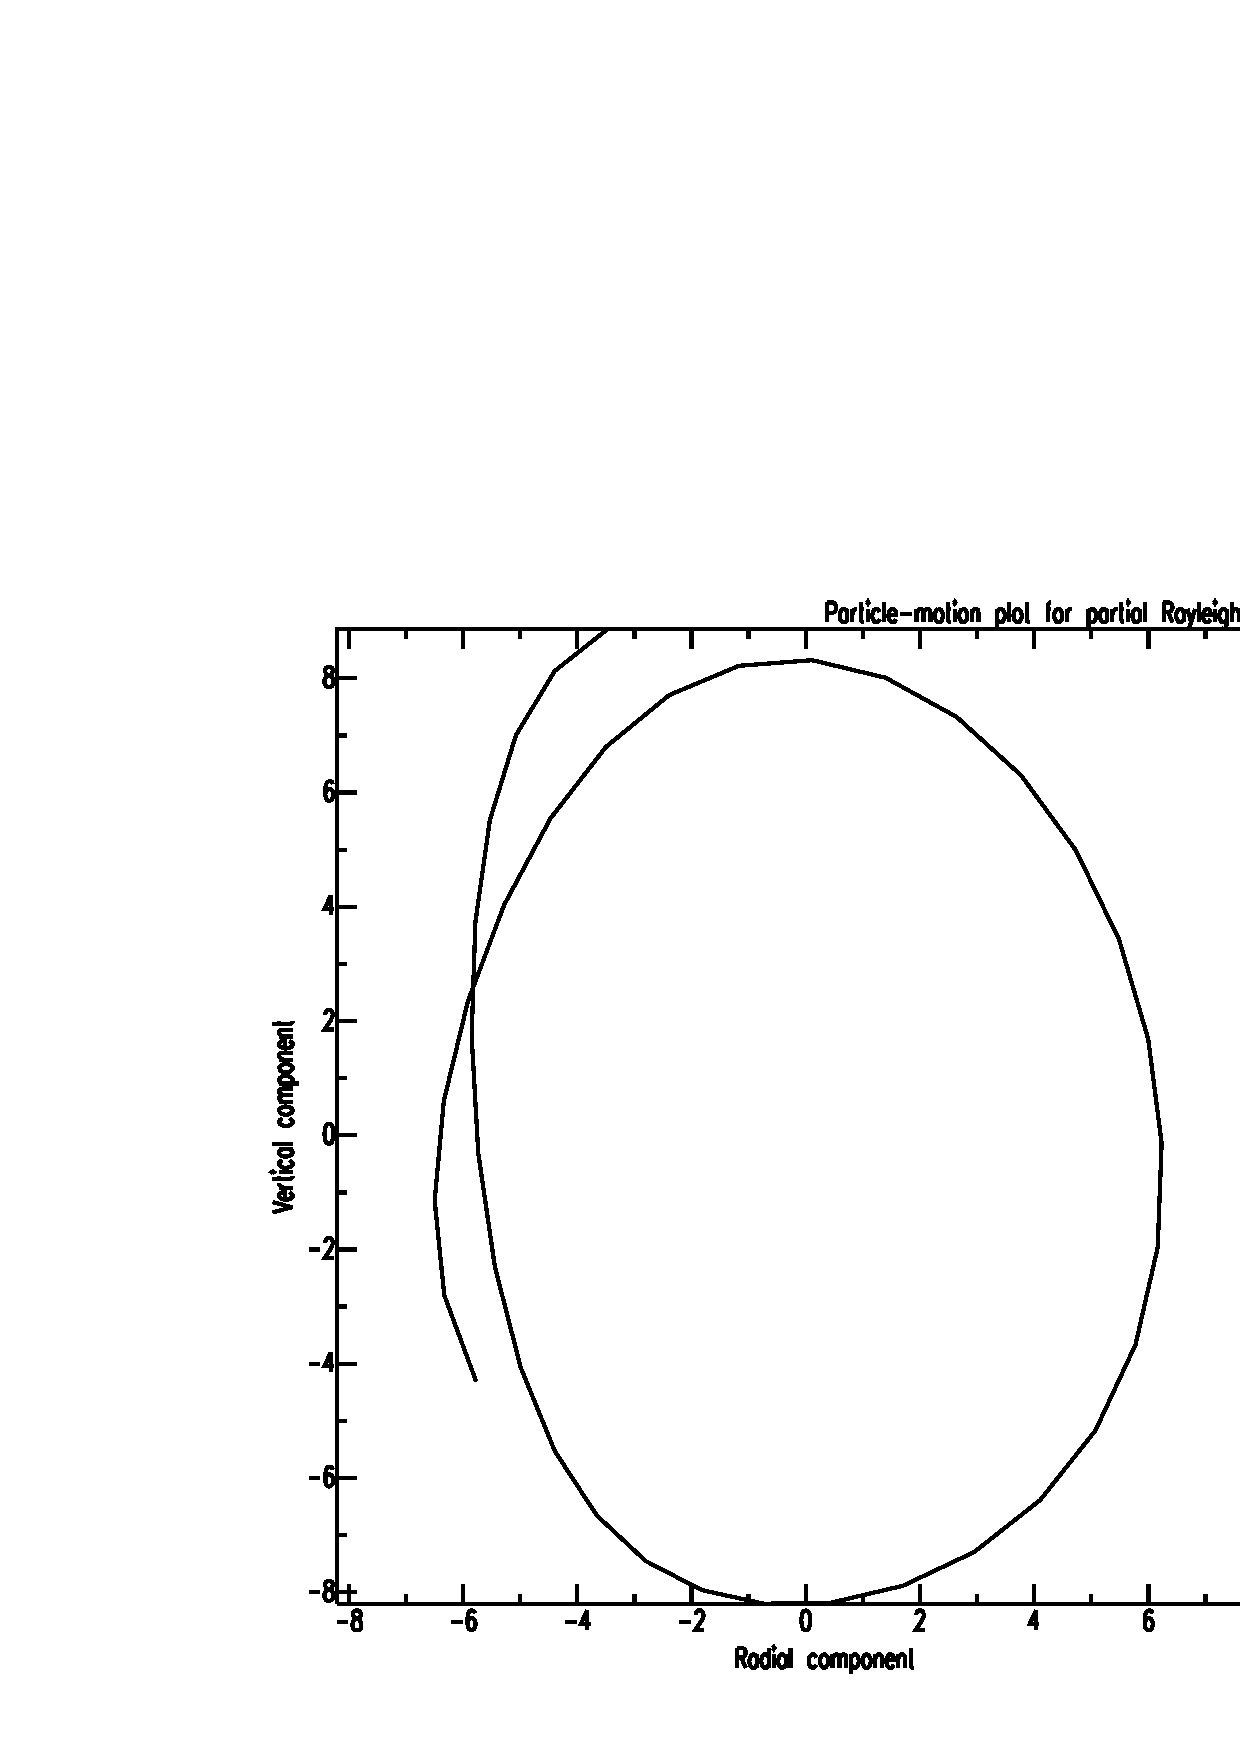
\includegraphics[width=\textwidth]{ppm}
\caption[质点运动图。]{Rayleigh面波的部分时间窗内的质点运动轨迹,为标准的逆进椭圆。}
\label{fig:ppm}
\end{figure}

\subsection{plotalpha}
\subsection{plotc}
\subsection{plotxy}
\subsection{plotdy}
\subsection{plotsp}
